% $Id$

\chapter{Regression dataset}
\label{data_example2}
\minitoc

This chapter will describe the steps necessary to perform a regression using PRoNTo. These are similar to the ones in the previous chapter, thus, the reader is advised to complete the tutorial in Chapter \ref{sec:Block_design_fMRI_dataset} before moving on, since the explanation of some steps will be less descriptive. The dataset used in this chapter can be found on PRoNTo's website \url{http://www.mlnl.cs.ucl.ac.uk/pronto/prtdata.html} (data set 3).


\section{GUI analysis}
As in Chapter \ref{sec:Block_design_fMRI_dataset}, the analysis of the data will start with the PRoNTo's GUI. Please create a folder in your computer to store the results and type `prt' or `pronto' on the \matlab{} command window. This will open the main interface of PRoNTo (see Figure \ref{fig:gui_main_screen} in the previous chapter).


%----------------------------------------------------------------------

\subsection{Data \& Design}

\begin{itemize}

	\item In PRoNTo's main window, click on `Data \& Design'. Like in the previous chapter, browse the directory in which to save the PRT structure (saved as `PRT.mat').
	
	\item In the panel `Groups', click on `Add' and provide a name to the group, e.g. `Aged'.

	\item Unlike the previous chapter, all the images in the dataset correspond to different subjects; therefore, click on the `Samples' tick box. This will lock the `Subjects/Samples' field, allowing you to skip to the third field.
	
	\item In the `Modalities' panel, click on `Add' and provide a name for the modality, e.g. `sMRI'.
	
	\item In the `Data format' choose the appropriate format for your data (here nifti); For other data formats the reader is referred to the tutorial of Chapter \ref{sec:multimodal_face}.
	
	\item You can see that the `Design' section is unavailable. Since we are doing a regression and every subject has only 1 sample/scan, there is no design matrix.
	
	\item Load all the image files available in the directory (IXIdata/aged/Guys/). You can select all the files by using the right mouse button and clicking on the option `Select All'. When all the images are selected, click on the `Done' button.
 
    \item Into the `Regression targets' field click `Specify Targets'. A new window will appear where you can either directly write (or paste) the list of target values, where in our case they are available in the `Age\_old\_Guys' file (IXIdata/aged/), or if you have a .mat file with the regression targets, you can select it directly by selecting the option `From .mat file' and choosing the appropriate .mat file. The two different options are shown in Figures \ref{fig:data_example2_gui_data_and_design_specify_targets_specify} and \ref{fig:data_example2_gui_data_and_design_specify_targets_mat_file}.

\begin{figure}[!h]
	\centering
	\begin{minipage}[b][6.3cm][b]{0.5\textwidth}
  \centering
	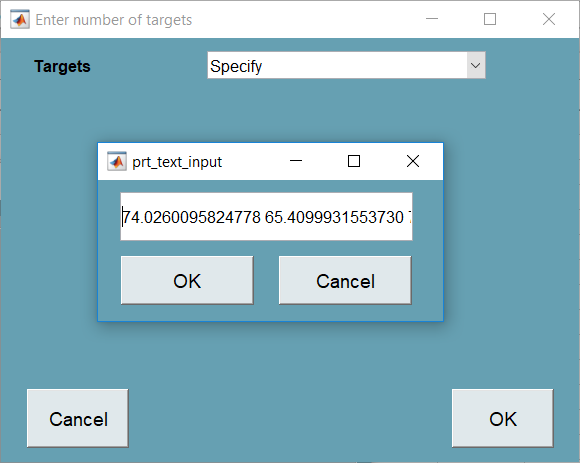
\includegraphics[scale=0.5]{images/Tutorial/v3/data_example2/data_example2_gui_data_and_design_specify_targets_specify.png}
		  \captionsetup{width=0.7\linewidth}
	\captionof{figure}{`Specify' option in the `Specify targets' GUI.}
	\label{fig:data_example2_gui_data_and_design_specify_targets_specify}
\end{minipage}%
	\begin{minipage}[b][6.3cm][b]{0.5\textwidth}
  \centering
	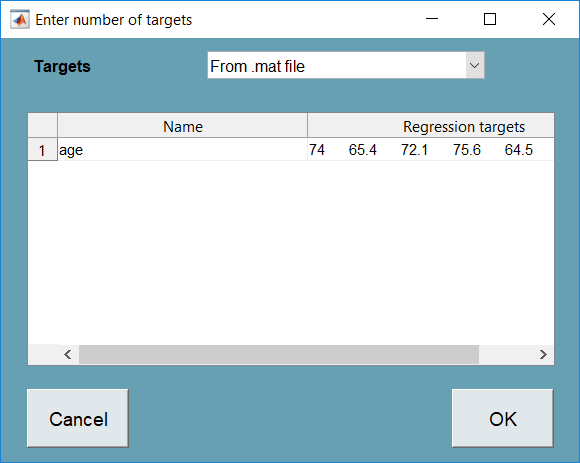
\includegraphics[scale=0.5]{images/Tutorial/v3/data_example2/data_example2_gui_data_and_design_specify_targets_mat_file.png}
		\captionsetup{width=0.7\linewidth}
	\captionof{figure}{`From .mat file' option in the `Specify targets' GUI.}
	\label{fig:data_example2_gui_data_and_design_specify_targets_mat_file}
	\end{minipage}
\end{figure}

     \item Leave the `Covariates' section as it is, and press `OK'. 

	 \item In the `Masks' field, on the bottom left of the `Data and design' window, select the `SPM\_mask\_noeyes' mask for the specified modality. The mask is available in the path where you have installed PRoNTo (PRoNTo/masks/).
    
     \item The `Data and design' window should look similar to Figure \ref{fig:data_example2_gui_data_and_design_final}. Click on the `Save' button to create `PRT.mat' file with the structure containing the information that has been previously specified. If no errors are shown in the \matlab{} command, leave the `Data and design' window by clicking `Quit'.

\begin{figure}[!h]
	\centering
		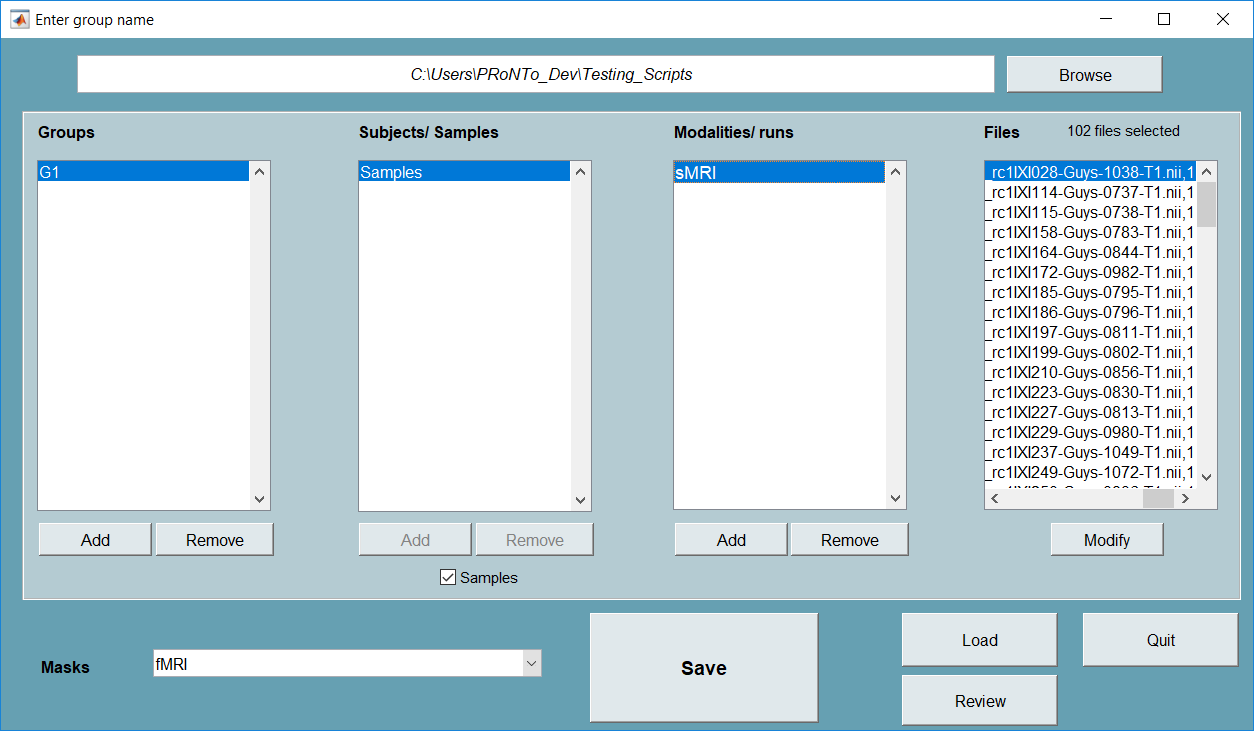
\includegraphics[scale=0.5]{images/Tutorial/v3/data_example2/data_example2_gui_data_and_design_final.png}
	\caption{`Data and design' GUI final configuration.}
	\label{fig:data_example2_gui_data_and_design_final}
\end{figure}

\end{itemize}

%----------------------------------------------------------------

\subsection{Prepare feature set}


\begin{itemize}

	\item In PRoNTo's main window, click on `Prepare feature set' and a new window will open prompting you to select a `PRT.mat' file. Select the `PRT.mat' file previously created in the `Data \& Design' step and you are now in the `Specify modality to include' window (see Figure \ref{fig:gui_prepare_featureSet_specify_modality} in the previous chapter). There is no need to change anything for this example. Just click on the `Done' button.
	
	\item Once you click on the `Done' button the window `Prepare feature set' will appear. Provide a name to the feature set, e.g. `Scalar\_Momentum'; and click on `Build Kernel / data matrix' to build the feature set and kernel.
	
\end{itemize}

%----------------------------------------------------------------

\subsection{Model: Specify new}
\begin{itemize}

    \item Next we have to specify a model. In PRoNTo's main window, click on `Specify new' and a new window will open, `Specify model' (see Figure \ref{fig:gui_specify_new} in the previous chapter).

   	\item Select the `PRT.mat' file and provide a name to the model, e.g. `KRR'.

    \item Select from the list one of the `Feature Set' previously defined. In this case, there is only one, `Scalar\_Momentum'.

	\item	Leave the option `Use kernels' tick box as it is, i.e. `Yes'.
	
	\item Select the `Regression' model type and click on the `Select subjects/scans` button. This will open a new window, `Specify subjects/scans to regress', click on the `Select all' button to use all the scans for the regression and `age' as our regression target (Figure \ref{fig:data_example2_gui_prepare_featureSet_select_subjects}). Current models available in PRoNTo do no enable multi-output prediction.
	
     \item Select the `Kernel Ridge Regression' option, in the Machine field.
     
	 \item Leave the option `Optimize hyper-parameter' tick box unchecked and `Cross-Validation Scheme' (internal loop) as it is. 
	
	\item Select the `Leave One Subject Out' cross-validation scheme (external loop).
	
	\item In the `Data operations' box, select only the `Mean centre features using training data' option. The final `Specify model new' window should look similar to the Figure \ref{fig:data_example2_gui_prepare_featureSet_final}. Click on the `Specify and run model' button.
	
    % \item Repeat the process two times using the other two machines. To do this, just follow the same steps in this section, but select the other options in the `Machine' drop-down list (`Relevance Vector Regression' and `Gaussian Process Regression') and give different names to the each model.


        %     \begin{figure}[h!]
        %     \begin{center}
        %         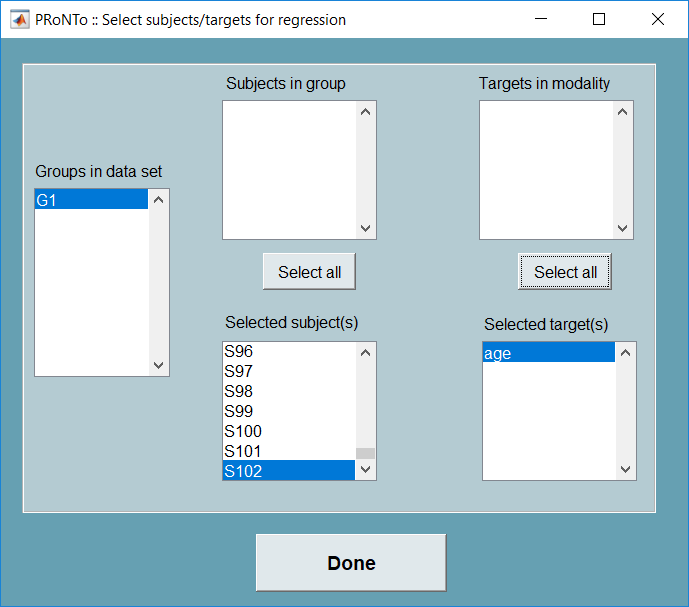
\includegraphics[scale=0.6]{images/Tutorial/v3/data_example2/data_example2_gui_prepare_featureSet_select_subjects.png}
        %     \end{center}
        %     \caption{`Specify subjects/scans to regress' GUI.}
        %     \label{fig:data_example2_gui_prepare_featureSet_select_subjects}
        % \end{figure}
    
        % \begin{figure}[h!]
        %     \begin{center}
        %         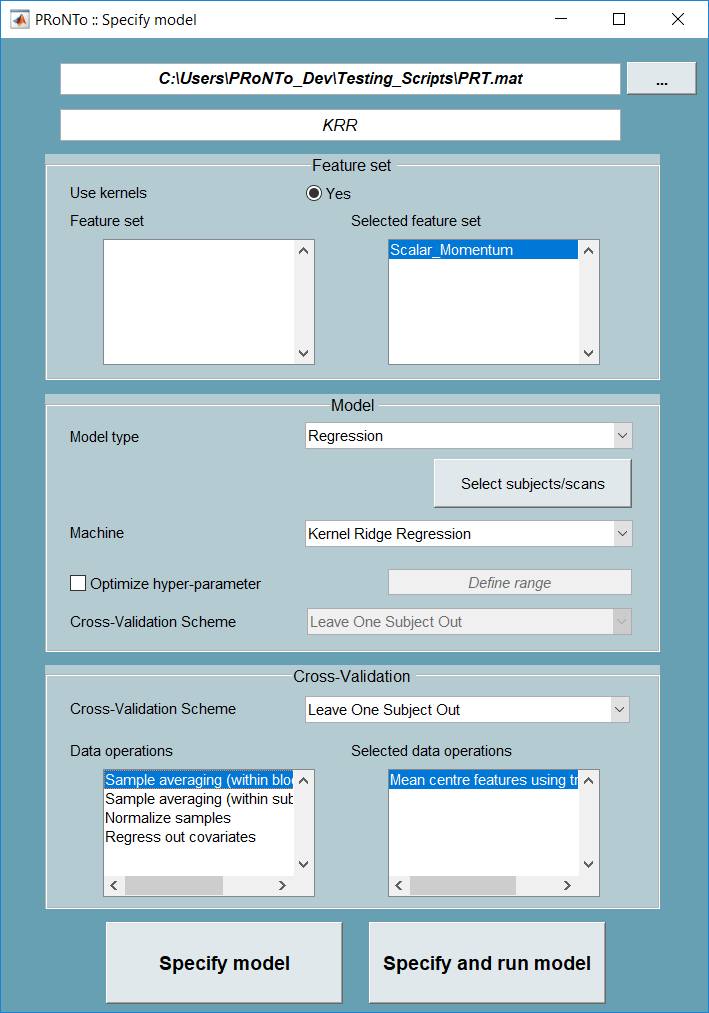
\includegraphics[scale=0.75]{images/Tutorial/v3/data_example2/data_example2_gui_prepare_featureSet_final.png}
        %     \end{center}
        %     \caption{`Specify model new' GUI final configuration.}
        %     \label{fig:data_example2_gui_prepare_featureSet_final}
        % \end{figure}
        
        
        
        \begin{figure}[!h]
	\centering
	\begin{minipage}[b][11.5cm][b]{0.5\textwidth}
  \centering
	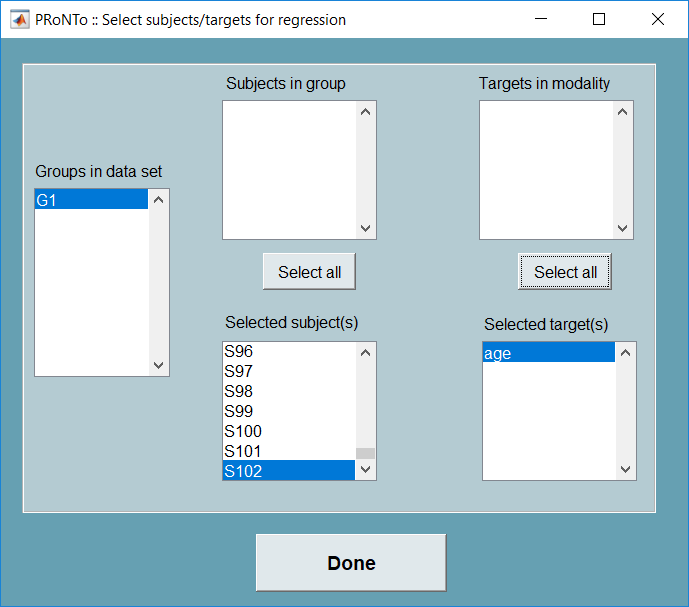
\includegraphics[scale=0.55]{images/Tutorial/v3/data_example2/data_example2_gui_prepare_featureSet_select_subjects.png}
		  \captionsetup{width=0.8\linewidth}
	\captionof{figure}{`Select subjects/scans' GUI.}
	\label{fig:data_example2_gui_prepare_featureSet_select_subjects}
\end{minipage}%
	\begin{minipage}[b][6.3cm][b]{0.5\textwidth}
  \centering
	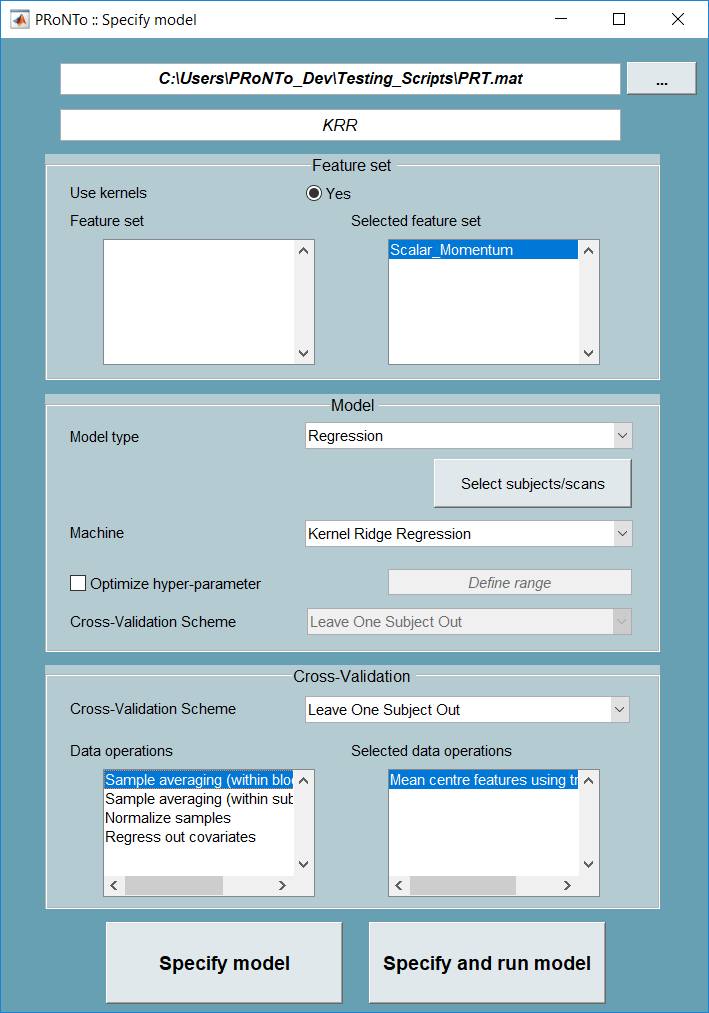
\includegraphics[scale=0.5]{images/Tutorial/v3/data_example2/data_example2_gui_prepare_featureSet_final.png}
		\captionsetup{width=0.7\linewidth}
	\captionof{figure}{`Model: Specify new' GUI.}
            \label{fig:data_example2_gui_prepare_featureSet_final}
	\end{minipage}
\end{figure}

\end{itemize}


%----------------------------------------------------------------------------

\subsection{Model: Specify from}

Use this module to copy the configurations of the previously defined KRR model but select the other options in the `Machine' drop-down list (`Relevance Vector Regression' and `Gaussian Process Regression') and give different names to each model. For further information regarding the `Model: Specify from' section the reader is referred to \ref{gui_specify_model_from} in the previous chapter and to chapter \ref{chap:ModelCrossV}.
        

%----------------------------------------------------------------------------

\subsection{Display results}
\label{sec:display_results_reg}
\begin{itemize}

    \item In PRoNTo's main window, click on `Display results' and select the `PRT.mat' file. This will open the main results window similar to the Figure \ref{fig:data_example2_gui_display_results}.

        \begin{figure}[h!]
            \centering
                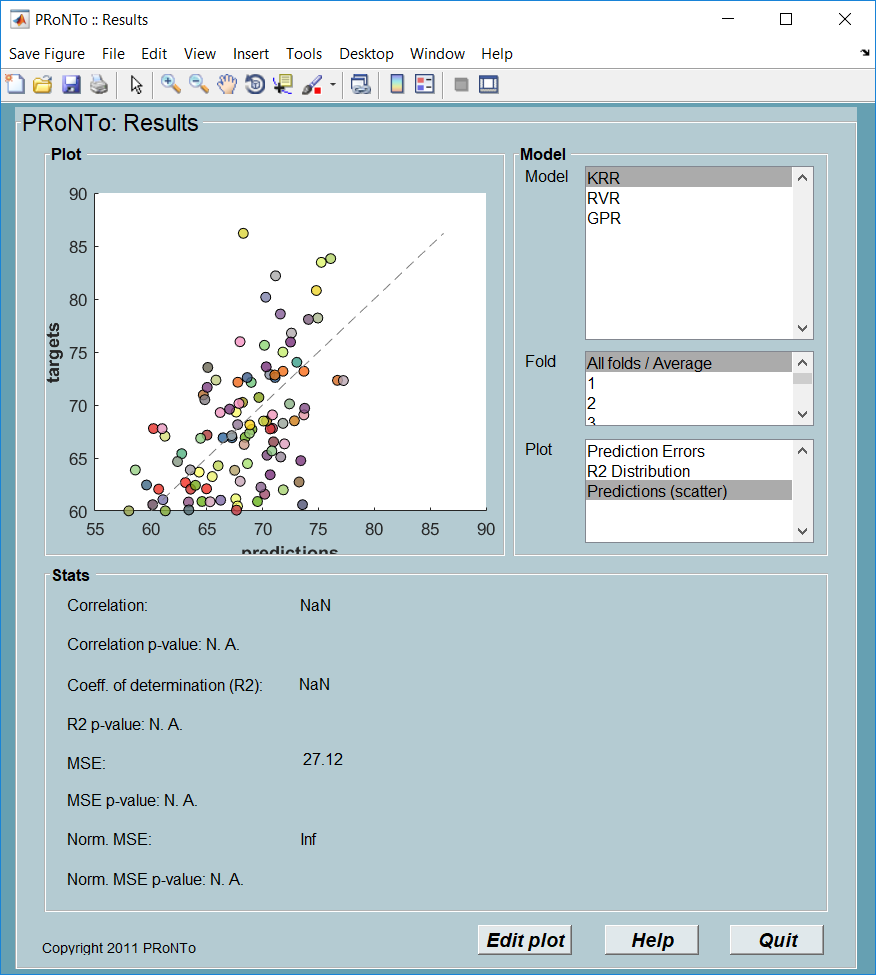
\includegraphics[scale=0.48]{images/Tutorial/v3/data_example2/data_example2_gui_display_results.png}
            \caption{`Display results' GUI.}
            \label{fig:data_example2_gui_display_results}
        \end{figure}

    \item In the `Results' window, one can select the different regression models in the `Model' list on the upper right panel. This will show the results obtained using each one of the regression models.
    
    \item Since we didn't run any permutation testing, the p-values of Correlation, R2, MSE and Normal MSE are not available. If one wants to check the statistical significance of the results, one should run his/her models from the `Model: Run' section of the main window, with permutation testing. For more detailed information the reader is referred to \ref{run_model}.
    
\end{itemize}


%=====================================================



%=====================================================

\section{Batch analysis}

In this section, the previous experiment will be repeated using the `\texttt{matlabbatch}' system. The reader is advised to complete the tutorial in Section \ref{batch_data_and_design} before continuing, since the explanation of each step will be less descriptive.

Once again, to analyse the data, create a new directory in which to save the results of the analysis. On the main interface of PRoNTo click on the `Batch' button to open the `{\tt matlabbatch}'. Alternatively, type `prt\_batch' in the \matlab{} prompt.

\subsection{Data \& Design}
\begin{itemize}

    \item Click on `Data \& Design' in the PRoNTo menu (see Figure \ref{fig:batch_data_and_design_full} in the previous chapter).
    
    \item In the `Directory' field, select a directory where the `PRT.mat' file will be saved.
    
    \item In the `Groups' field:
 	
		\begin{itemize}
		
		\item Add one group.
		
		\item In the field `Name', provide a name without spaces for this group, e.g. `Aged'.

    	\item In the field `Select by', select the `Samples' option and add a new modality. For more information on the Samples option please consult Chapter \ref{chap:DataDesign}.
        	
    	\item Provide a name for this modality, e.g. `sMRI' and choose the appropriate data format (here nifti).
    	
    	\item Select the image files available in the `aged/Guy' directory of the IXI dataset.
    	
    	\item In the `Regression targets (subject)' option specify the regression targets by selecting the `Age\_old\_Guys' .mat file (IXIdata/aged/).
    	
    	\item Leave `Covariates' field as default.

\end{itemize}    

		\item In the `Masks' field, add a new modality and provide the same modality name, `sMRI'; choose the appropriate data format, and select the `SPM\_mask\_noeyes' mask available in the path where you have installed PRoNTo (PRoNTo/masks/). The name of the modality here has to be exactly the same as in `Modalities', otherwise it will not work.
		
    \item Leave the `HRF overlap' and the `HRF delay' fields as default.
	
	\item In the `Review' field, select `Yes' if you would like to review your data and design in a separate window. Otherwise, leave as it is, i.e. `No'.
        
\end{itemize}

Figure \ref{fig:data_example2_batch_data_and_design_final} is the final configuration of the {\tt matlabbatch} `Data \& design' module.

        \begin{figure}[h!]
            \centering
                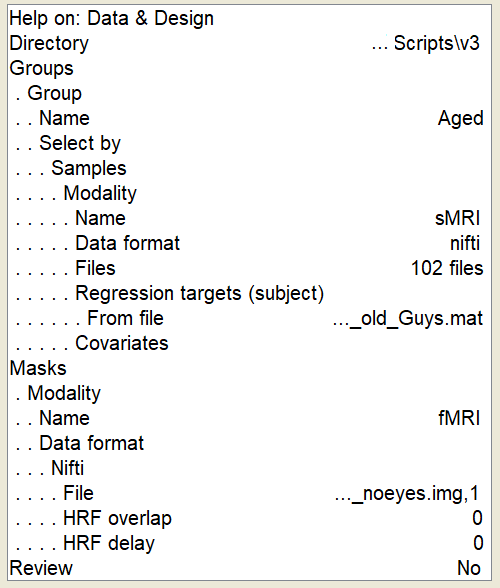
\includegraphics[scale=0.5]{images/Tutorial/v3/data_example2/data_example2_batch_data_and_design_final.png}
            \caption{Data \& design module in {\tt matlabbatch}.}
            \label{fig:data_example2_batch_data_and_design_final}
        \end{figure}
        
%---------------------------------------------------------------

\subsection{Feature set / Kernel}

\begin{itemize}

    \item Click on the `Feature set / Kernel' option on PRoNTo's {\tt matlabbatch} menu.
    
     \item With `Load PRT.mat' field selected, click on the `Dependency' button to associate the `PRT.mat' file created in the previous `Data \& Design' step or click on the `Select files' button to browse where `PRT.mat' file was saved.

    \item Provide a name to the `Feature/kernel' set, e.g. `Scalar\_Momentum'.
    
    \item Select the `Nifti' option for a data format, add one modality and select the modality name with the `Dependency' button\footnote{Or type it in manually, `sMRI', but the name needs to be {\it exactly} the same as the one specified in the `Data \& Design' module.}(Data \& Design:Mod\#1 name).
	
		\begin{itemize}
	
	\item In the `Samples/Conditions' field, select `All samples' option.
	
	\item In the `Voxels to include' field, select `All voxels' option, this means we are not entering with an additional second-level mask.
	
	\item In the `Detrend' field, select the `None' option.
	
	\item In the `Scale input scans' field, select the `No scaling' option and finally leave `Use atlas to build ROI specific kernels' as default.
	
	\end{itemize}

	\item Figure \ref{fig:data_example2_batch_prepare_featureSet_final} is the final configuration of the {\tt matlabbatch} `Feature set / Kernel' module. For the other Data formats the reader is referred to chapter \ref{chap:ModelCrossV}.

\begin{figure}[h!]
	\centering
		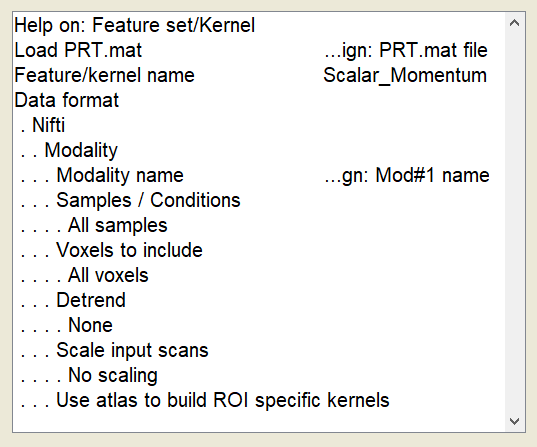
\includegraphics[scale=0.6]{images/Tutorial/v3/data_example2/data_example2_batch_prepare_featureSet_final.png}
	\caption{Feature set / Kernel module. Selected parameters in the Modality option.}
	\label{fig:data_example2_batch_prepare_featureSet_final}
\end{figure}
    
\end{itemize}

%----------------------------------------------------------------------

\subsection{Model: Specify new (KRR)}
\label{ssec: model_spec_new_krr}


\begin{itemize}

\item Click on the `Model: Specify new' option on PRoNTo's {\tt matlabbatch} menu.

\item With `Load PRT.mat' field selected, click on the `Dependency' button to associate the `PRT.mat' file created in the previous `Feature set / Kernel' step or click on the `Select files' button to browse where `PRT.mat' file was saved.

\item Provide a name to the model, e.g. `KRR'.

\item Select the feature set name with the `Dependency' button\footnote{or write it {\it exactly} as previously defined in the `Feature set / Kernel' module (option `Feature set/Kernel: Feature/kernel name'), here `Scalar\_Momentum'.}. From v3.0, multiple feature set is supported so you can put more than one feature set names.
    
\item Select the `Regression' model type:

    \begin{itemize}
    
    \item Add a new group and call it `Aged'.
    
    \item In the `Subjects' field, type `1:102'. This will instruct the program to use all the 102 scans, i.e. from scan 1 to scan 102.
    
    \item In the `Conditions / Samples' choose `Target' and type in `age', as this is the name of our regression target variable in the `Age\_old\_Guys.mat' file.
       
    \end{itemize}
    
    \item In the `Machine' field: 
    
    \begin{itemize}

   \item Select `Kernel machine' and then select the `Kernel Ridge Regression' option:
       
	\item In the `Machine optimization and parameters', select `No optimization', and leave `No optimization' as it is, i.e. `1'.

   \end{itemize}
   
   \item In the `Cross-validation type' field, select `Leave One Subject Out' option.
	
	\item Leave the `Include all scans' field as it is, i.e. `No'.

	\item In the `Data operations' field:
	
		\begin{itemize}
		\item  Leave the `Mean centre features' field as it is, i.e. `Yes'. 
				
		\item  Leave the `Other Operations' field as it is, i.e. `No operations'.
		\end{itemize}
	
\end{itemize}

The final configuration of the of the {\tt matlabbatch} `Model: Specify new' module should look similar to Figure \ref{fig:data_example2_batch_model_specify_new_final}.

\begin{figure}[h!]
	\centering
		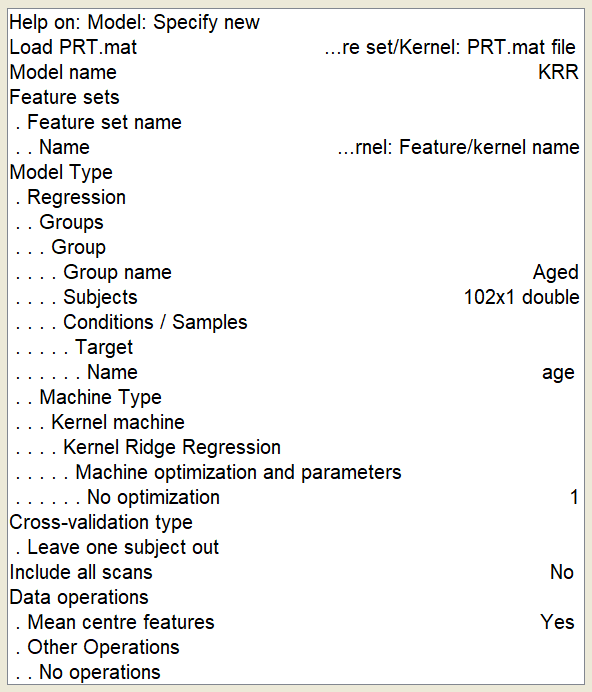
\includegraphics[scale=0.5]{images/Tutorial/v3/data_example2/data_example2_batch_model_specify_new_final.png}
	\caption{`Model: Specify new' module in {\tt matlabbatch}, final configuration.}
	\label{fig:data_example2_batch_model_specify_new_final}
\end{figure}


%---------------------------------------------------------------------------------

\subsection{Model: Run (KRR)}

\begin{itemize}

    \item Click on the `Run model' option on PRoNTo's {\tt matlabbatch} menu.
    
   	\item  With `Load PRT.mat' field selected, click on the `Dependency' button to associate the `PRT.mat' file created in the previous `Specify model' step.

    \item Select the model name from the `Specify model' module with the `Dependency' button\footnote{or write it {\it exactly} as previously defined in the `Specify model' module, here `KRR'}.
    
    \item In the field `Do permutation test?', leave as it is, i.e. `No permutation test' 

       \end{itemize}

\subsection{Model: Specify and Run (RVR and GPR)}

The specification of the other models (`Relevance Vector Regression' and `Gaussian Process Regression') can be done using the `Specify from' module. The only difference is that in the `Machine' field of the `Specify from' module, one has to choose the appropriate machine to use (`Relevance Vector Regression' or `Gaussian Process Regression'). The parameters used for each machine should be the default ones.

Note that when the `PRT.mat' file is loaded in each module, the user should select the latest option on the list.

When all the models are defined, the `Module List' should contain 8 modules:
\begin{enumerate}
    \item Data \& Design.
    \item Feature set/Kernel.
    \item Mode: Specify new.
    \item Mode: Run.
    \item Mode: Specify from.
    \item Mode: Run.
    \item Mode: Specify from.
    \item Mode: Run.
\end{enumerate}

Note that modules 3 and 4 correspond to the KRR model; 5 and 6 to the RVR model; 7 and 8 to the GPR model.

When all the modules are added, just click on the `Run Batch' button. The resulting `PRT.mat' file will be saved in the specified directory and the results can be viewed using the process described in Section \ref{sec:display_results_reg}.



\section{Removing confounds (optional)}

In this tutorial until now we only had subjects from a specific testing  site. Say now that in your study this isn't true. For example in the IXI study there were 3 testing sites, Hammersmith Hospital using a Philips 3T system, Guy’s Hospital using a Philips 1.5T system and the Institute of Psychiatry using a GE 1.5T system. What changes? How could we account for the potential differences of the scanner systems? One way to do it is by `regressing out the covariates'. Please see section \ref{sec:Covariates} for important considerations on covariates.
\\
Chapter \ref{sec:confounds_clas} is a detailed tutorial about removing confounds in a classification example, so the reader is strongly advised to go through that tutorial first and if one is interested to try a regression example as well, one should come back here afterwards as this is not a complete tutorial regarding removing confounds.
\\

The first main thing that one has to change is in the `Data \& design' module.

\begin{itemize}
    
    \item In the `Files', you need to select all 170 subjects from all the 3 different folders (representing one testing site each).
    
    \item In the `Covariates' field, you need to type the covariates you want to regress out. Covariates can be input to PRoNTo by directly copying values into the Covariate if there is only one confounding factor (e.g. a continuous confound), or by typing the full path of the {\tt R} matrix containing either one column or multiple columns. As `Testing site' is categorical, one-hot encoding was used (i.e. one column for each testing site in the `R' matrix). In this example, you need to select the file Confounds/\_one/\_hot.mat found in the IXI/Data/aged/ folder.
    
    \end{itemize}
    
The second important thing is in the `Specify model new' module.
    
    \begin{itemize}
    
    \item Select the `Kernel Ridge Regression' option in the Machine field. You can also do the same procedure choosing `Gaussian Process Regression' if you want to try more than one machines.
	
	 \item Check the option `Optimize hyper-parameter' tick box. Type `10.\textasciicircum{}[-5:5]' on the right field. Then, select `k-fold CV on Subject-Out' option in the `Cross-Validation Scheme' field (internal loop), and type `5' in the new window that will open.
	
	\item Select the `Leave One Subject Out' cross-validation scheme (external loop).
	
	\item Now here comes the important part, where we specify that we want to regress out covariates. In the `Data operations' box, first select the `Mean centre features using training data' option as we are doing so far. But now also select the `Regress out covariates (subject level)' option, which corresponds to the removal of the contribution of some external variables to the data. Click on the `Specify and run model' button.
	
\end{itemize}

If you now wish to find the effects of removing the covariates, you have to rerun a new model exactly the same with the previous one, but without regressing out the covariates in the `Data operations' box, and compare the differences in the performance measures.









\section{Within- and between- subject regression}

As mentioned sporadically throughout the whole PRoNTo Manual, until PRoNTo v2.1, the user could only input one regression target per subject. Thus, the option of doing within-subject regression was not available, and between-subject regression could only be done with one regression target.
\\

From PRoNTo v3.0, multiple regression targets can be specified at the Data \& Design level (although they can only be modelled independently, i.e. one regression model per target). The new functionalities in this version, enable users to specify both which target and which samples (i.e. which subjects for between-subject regression or which trials for within- subject regression) to use for the regression model.
\\

The user is referred to Part \ref{sec:part_1} for further information regarding this topic.



